\yesmargins
\chapter{Cognitive Style Heuristics}
\begin{tikzpicture}[overlay,remember picture] 
\node[anchor=south] at ([yshift=5in,xshift=2.1in]current page text area.south){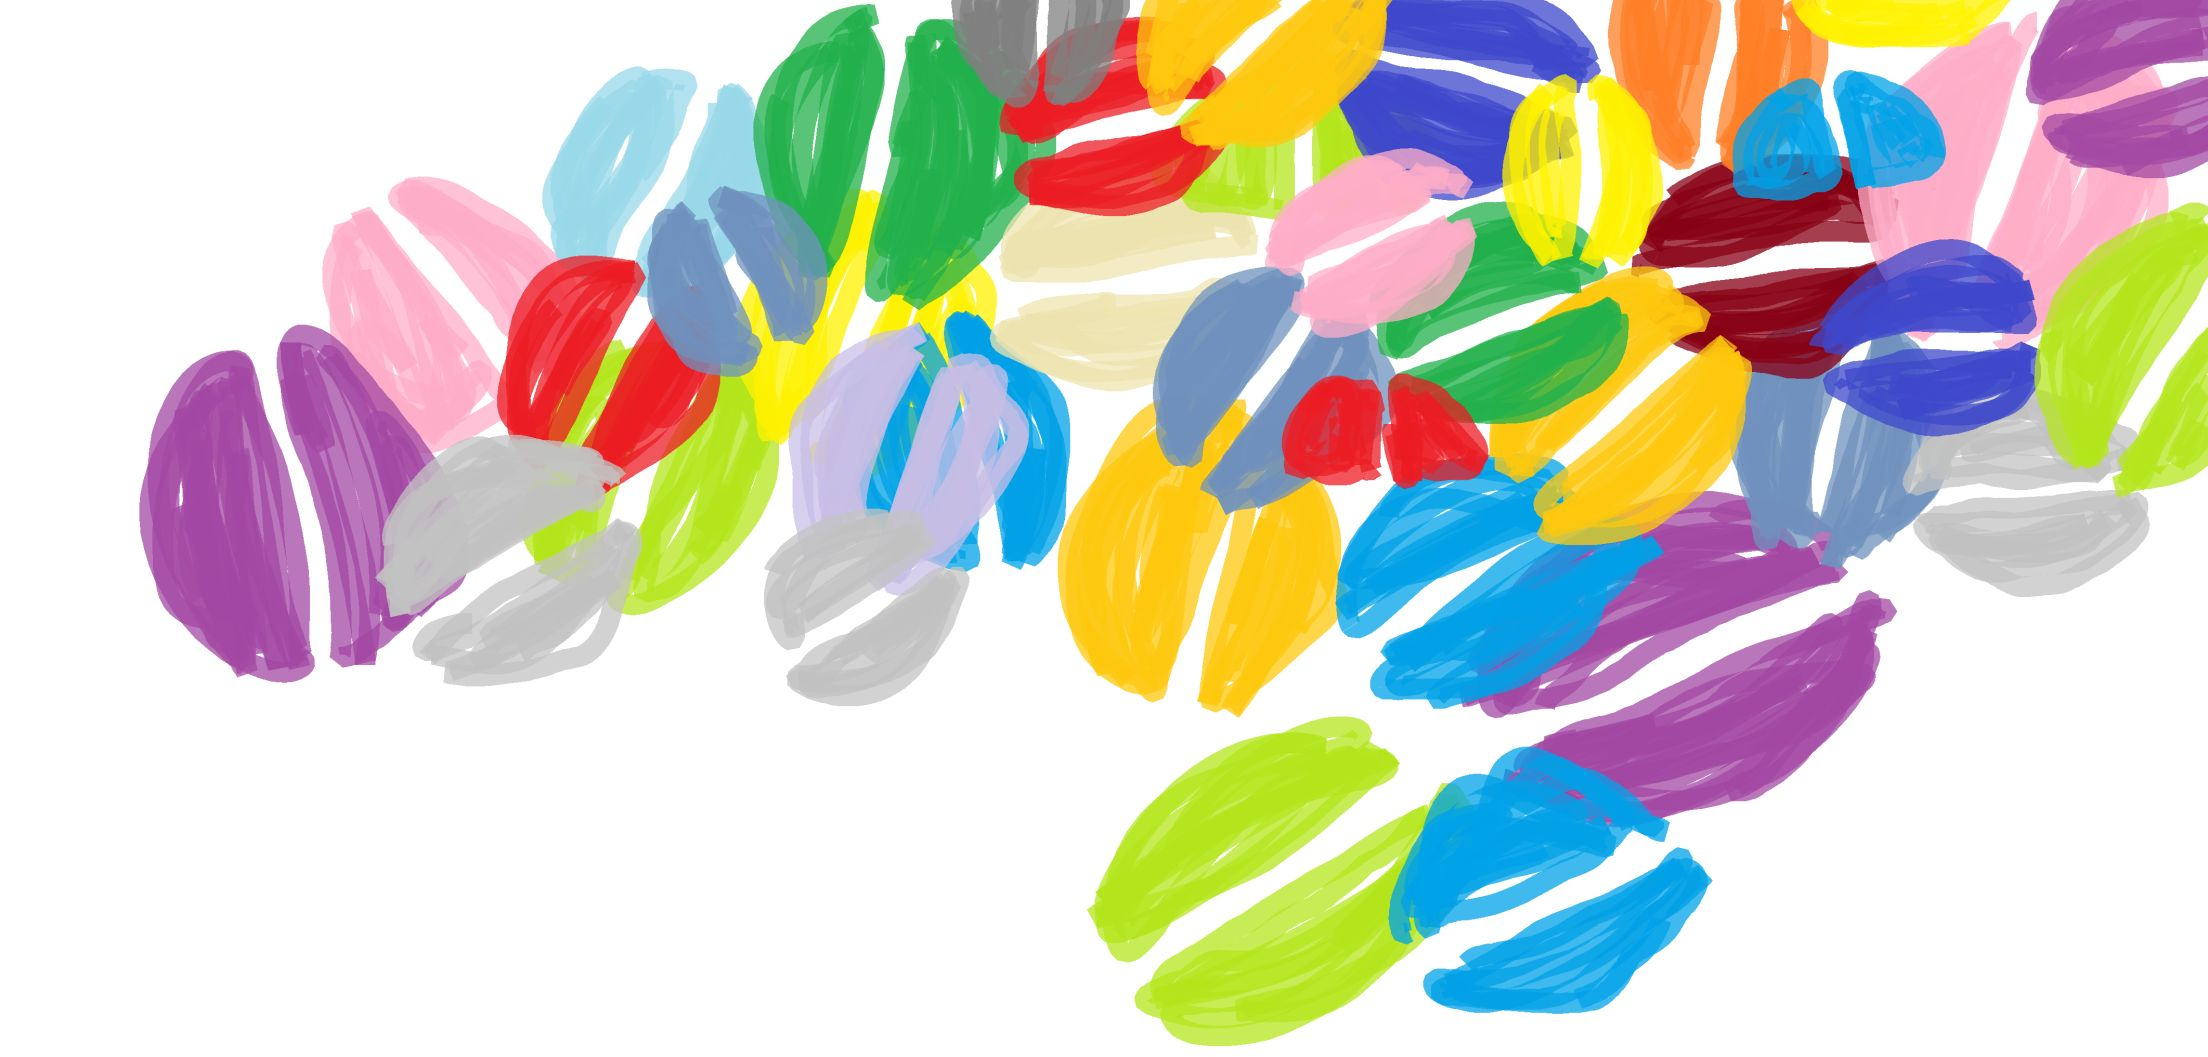
\includegraphics[width=11.5in]{csh02-sm}}; 
\end{tikzpicture}\marginpar{\textbf{Cognitive Style Heuristics (CSH)\index{cognitive style heuristics}}: Eight principles of interaction design\index{interaction design} for finding and fixing usability\index{usability} bugs in software. They are based around different cognitive styles\index{cognitive styles} different people use when they problem-solve in software.\margindivider}\marginpar{\textbf{interaction design}\index{interaction design}: An approach to technology design that involves helping users understand what's happening with the technology, what just happened, and what they can do \parencite{norman13}.}The \textbf{Cognitive Style Heuristics (CSH)}\index{cognitive style heuristics} are eight principles of \textbf{interaction design}\index{interaction design} used to improve software usability\index{usability}. They are framed around how different people use software in different ways. The CSH\index{cognitive style heuristics} were created by a research team headed by Margaret Burnett, one of the world's leading experts in usability research and \textbf{inclusive software design}.

The CSH\index{cognitive style heuristics} were created with new users in mind: People who have never seen, interacted with, or received previous direction on the software. They can also improve usability for more seasoned users who have figured out how to use the software to complete their tasks but may still be unhappy with the software.

\section{Cognitive Style Facets}\marginpar{\textbf{inclusive software design}: A type of software user interface design with the goal of increasing usability for traditionally under-served user populations while also increasing usability for mainstream users.\margindivider}\marginpar{\textbf{cognitive style facets (CSFs)\index{cognitive style facets}}: Five aspects of users that affect how they solve problems in software: Motivations\index{motivations (cognitive style facet)}, information processing style\index{information processing style (cognitive style facet)}, computer self-efficacy\index{computer self-efficacy (cognitive style facet)}, attitude toward risk\index{attitude toward risk (cognitive style facet)}, learning style\index{learning style (cognitive style facet)}\margindivider}\marginpar{\textbf{motivation CSF\index{motivations (cognitive style facet)}}: Why someone is using the software (task completion vs. interest)\margindivider}\marginpar{\textbf{information processing style CSF\index{information processing style (cognitive style facet)}}: How a person looks through or absorbs information in software (comprehensively vs. selectively)\margindivider}\marginpar{\textbf{motivation CSF}: Why someone is using the software (task completion vs. interest)\margindivider}\marginpar{\textbf{computer self-efficacy CSF\index{computer self-efficacy (cognitive style facet)}}: A person's confidence in their ability to use computers or software (low vs. high)}

At the core of the Cognitive Style Heuristics\index{cognitive style heuristics} are the \textbf{cognitive style facets}\index{cognitive style facets}, five aspects of human cognition that affect how users problem-solve in software:

\begin{enumerate}
\item{\textbf{Motivations} for using software (task completion vs. tech interest). A person who is feeling task-motivated might choose to use software because they have something specific they need to accomplish, and might focus on that task immediately when they open the software and the whole time they're using it. A person who is feeling interested in the software itself might seek out the new and exciting features and spend a lot of time exploring them.}

\item{\textbf{Information processing style} (comprehensive vs. selective). A person processing comprehensively might want to understand details, implications, or to get a sense of overall structure before taking action in software. A person processing selectively might take action as soon as they detect what seems like the beginning of a promising path.}
\item{\textbf{Computer self-efficacy} (low vs. high). A person who is feeling low computer self-efficacy might think it's their fault when they make a mistake or encounter a problem in the software. A person feeling high computer self-efficacy might feel the software is poorly made if they make a mistake or encounter a problem in the software.}
\item{\textbf{Attitude toward risk} (risk-tolerant vs. risk-averse). A person who is feeling risk-averse might avoid taking actions that have unknown consequences or seem dangerous or irreversible. A person who is feeling risk-tolerant might take actions even if they know those actions could lead to bad consequences.}
\item{\textbf{Learning style} (tinkering vs. by process). When someone is tinkering, they might click a button just because it's clickable then learn from what happens. When someone is learning by process, they might seek a logical first step, and want to proceed smoothly from start to finish.}
\end{enumerate}

As you probably noticed, each of the cognitive style facets has two polar \textbf{cognitive style facet values} (or \textbf{cognitive styles}\index{cognitive styles}). Each pair of facet values creates a spectrum. When each of us uses software, the way we feel and behave corresponds to somewhere on each of those spectra. Our individual facet values may be similar each time we use software, but they can also vary by context and change over time. For example, many people feel cognitively impatient when reading paragraphs of text (``text walls'') on websites and might process them more selectively, whereas they might want to catch every word of a new novel by their favorite author (comprehensive processing). \marginpar{\textbf{attitude toward risk CSF}\index{attitude toward risk (cognitive style facet)}: How willing a person is to take chances in software (risk-tolerant vs. risk-averse)\margindivider}\marginpar{\textbf{learning style CSF}: How a person prefers to move through software (tinkering vs. by process)\margindivider}\marginpar{\textbf{cognitive style facet value (A.K.A., cognitive style)}: A position on the spectrum of a cognitive style facet\margindivider}\marginpar{\textbf{persona}\index{persona}: A fictional character that represents a subset of users in a target audience. Personas are used in marketing and UI design to help with focusing on particular groups of users and customers \parencite{pruitt10,martin12}.\margindivider}\marginpar{\textbf{cognitive style personas}: Three specialized personas (Abi, Pat, and Tim) used for making software UI designs more usable to people with different cognitive styles.}

\section{Cognitive Style Personas}

The CSH are stated from the perspective of improving usability for the three \textbf{cognitive style personas}: Abi, Pat, and Tim. A \textbf{persona}\index{persona} is fictional person that is created to represent a group of users within a target audience. Personas are used to help marketing teams keep important subsets of their target audience in mind, and in software UI design for the same reason. Personas are typically documents that include a photo, name, age, gender, other background information, and information about how the made-up person interacts with product or software.

The cognitive style personas have a similar purpose but are distinct from traditional personas in multiple ways:
\begin{itemize}
\item{There are three and only three (Abi, Pat, and Tim).}
\item{Abi, Pat, and Tim each have a different set of cognitive styles. The cognitive styles are fixed.}
\item{Abi, Pat, and Tim are each multi-personas: They each have multiple photos of different people who appear to be of different ages, races, genders, etc.}
\item{Abi, Pat, and Tim were specifically created for evaluating \textit{software} (not marketing).}
\item{Abi, Pat, and Tim represent different positions on the cognitive style facet spectrum: Abi and Tim are on the ends and Pat is in the middle.}
\end{itemize}

The idea of the cognitive style personas is that creating software that works well for Abi and Tim (the two ends of the cognitive style facet value spectrum) will result in software that's better for them and everyone in between.

\nomargins
\subsection{Abi, Pat, and Tim}

\begin{tcolorbox}[colback=abicolor!100!white,colframe=abicolor2!100!black]
{\Large \textbf{Abi (Abigail/Abishek)}}\\
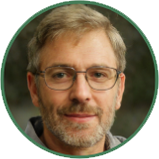
\includegraphics[scale=0.5]{abi1}
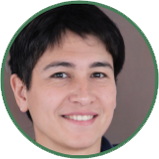
\includegraphics[scale=0.5]{abi3}
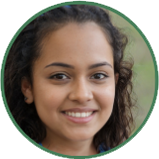
\includegraphics[scale=0.5]{abi2}\\
\textbf{Motivation}: Uses technology to accomplish their tasks.\\
\textbf{Computer self-efficacy}: Lower self-confidence than their peers about doing unfamiliar computing tasks. Blames themselves for problems.\\
\textbf{Attitude toward risk}: Risk-averse about using unfamiliar technologies that might require a lot of time\\
\textbf{Information processing style}: Comprehensive\\
\textbf{Learning style}: Process-orientated learning
\end{tcolorbox}

\begin{tcolorbox}[colback=patcolor!100!white,colframe=patcolor2!100!black]
{\Large \textbf{Pat (Patricia/Patrick)}}\\
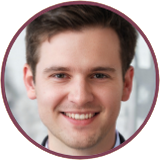
\includegraphics[scale=0.5]{pat2}
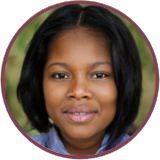
\includegraphics[scale=0.5]{pat1}
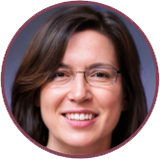
\includegraphics[scale=0.5]{pat3}\\
\textbf{Motivation}: Learns new technologies when they need to\\
\textbf{Computer self-efficacy}: Medium confidence doing unfamiliar computing tasks. If a problem can't be fixed, they will keep trying\\
\textbf{Attitude toward risk}: Risk-averse and doesn't want to expend time when they might not receive benefits\\
\textbf{Information processing style}: Comprehensive\\
\textbf{Learning style}: Likes to explore and purposefully tinker
\end{tcolorbox}

\begin{tcolorbox}[colback=timcolor!100!white,colframe=timcolor2!100!black]
{\Large \textbf{Tim (Timara/Timothy)}}\\
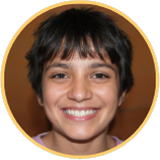
\includegraphics[scale=0.5]{tim1}
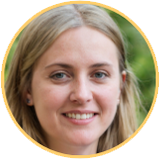
\includegraphics[scale=0.5]{tim3}
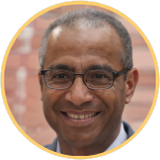
\includegraphics[scale=0.5]{tim2}\\
\textbf{Motivation}: Likes learning all the available functionality on all their devices\\
\textbf{Computer self-efficacy}: High confidence in technical abilities. If a problem can't be fixed, blame goes to software vendor.\\
\textbf{Attitude toward risk}: Doesn't mind taking risk using features of technology\\
\textbf{Information processing style}: Selective\\
\textbf{Learning style}: Likes tinkering and exploring
\end{tcolorbox}

\section{The Heuristics}

Note: The designs shown below were modelled after examples found in published software.

\subsection{Heuristic \#1 (of 8): Explain the \textit{benefits} of using new and existing features}

\begin{itemize}
\item Abi and Pat are motivated to use tech only as needed for their task. They rarely have spare time and prefer familiar features so they can keep focused on the task. Unless they see how features will help with their task, they may not be interested in using them.
\item Abi is risk-averse with tech. For example, they may avoid using features that have an unknown time cost and other unknown risks.
\item Pat is also risk-averse with tech, but might try out the features to determine whether they are relevant to accomplishing their task.
\item Tim likes learning what features can help them accomplish and is motivated to investigate new, cutting-edge features. Tim is also risk-tolerant so may use features without knowing their cost or even what they do.
\end{itemize}

\noindent To support their \textbf{motivations} and \textbf{attitudes toward risk}, allow Abi and Pat to quickly assess the benefits of features so they can choose whether to use them. Allow Tim to quickly assess which features are new and unique and what the features do so they can explore it if desired.

\spacer
\noindent\textbf{Example 1: Each featured extension has a brief description that says what the extension does and why somebody would use it.}
\begin{center}
\noindent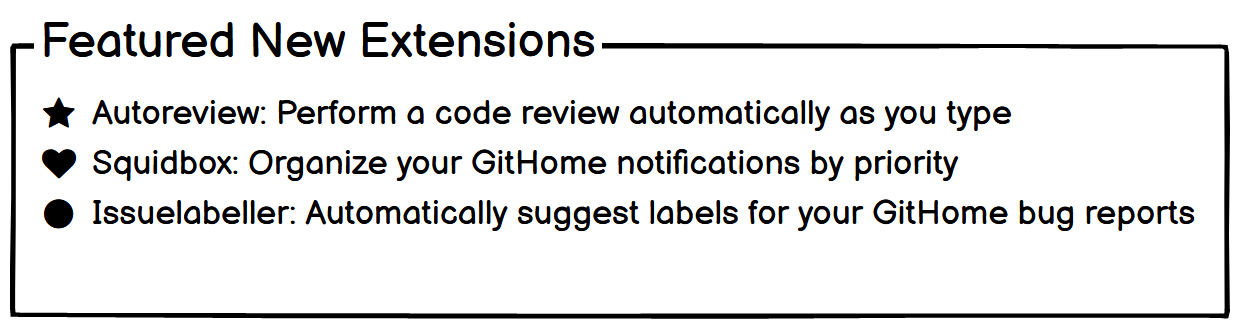
\includegraphics[width=0.95\textwidth]{h1-03}
\end{center}

\noindent\textbf{Example 2: Announcement briefly describes a new feature and how to use it.}
\begin{center}
\noindent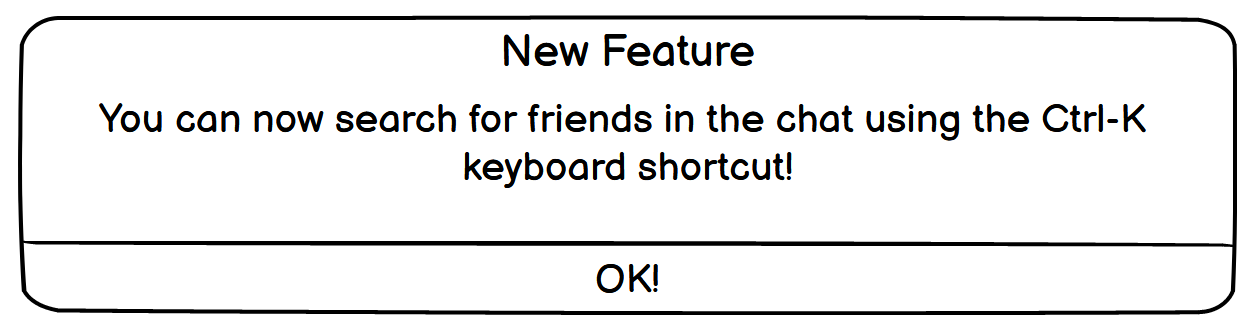
\includegraphics[width=0.95\textwidth]{h1-04}
\end{center}

\noindent\textbf{Example 3: Tooltip says why someone might use the search.}
\begin{center}
\noindent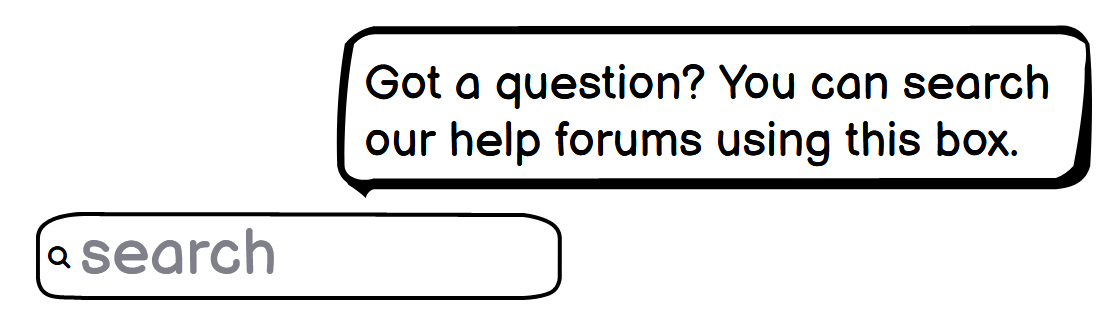
\includegraphics[width=0.7\textwidth]{h2-03}
\end{center}

\noindent\textbf{Example 4: Each tile explains a feature and the benefit of using the feature.}
\begin{center}
\noindent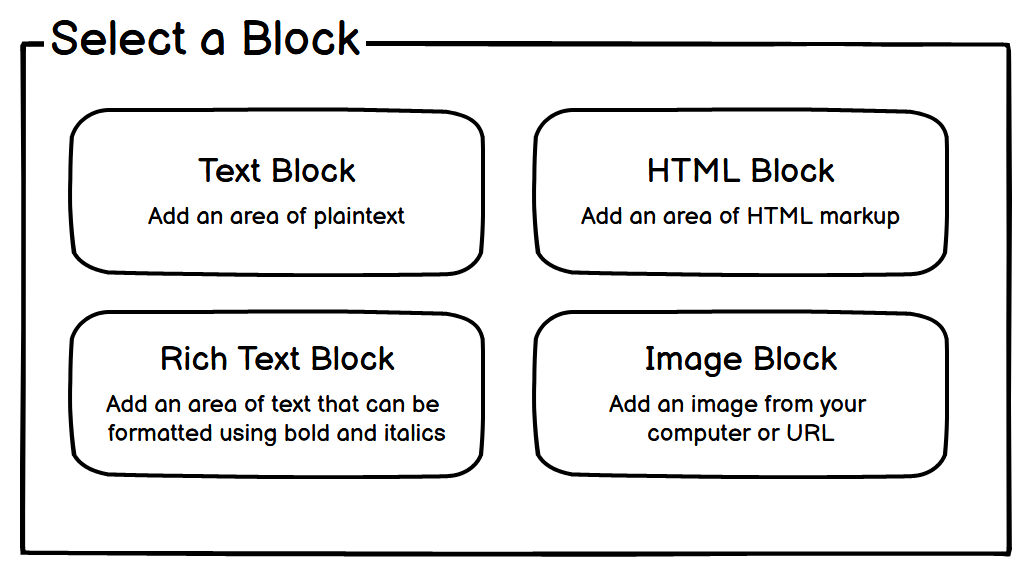
\includegraphics[width=0.95\textwidth]{h2-04}
\end{center}

\subsection{Heuristic \#2 (of 8): Explain the \textit{costs} of using new and existing features}

\begin{itemize}
    \item Abi and Pat are risk-averse, so they may want to avoid features with high effort costs if the benefits of using these features are unclear.
    \item Tim is risk-tolerant, so may begin using features that require extra effort and time, and that are unrelated to the task at hand.
\end{itemize}

\noindent To support their \textbf{attitudes toward risk}, allow Abi and Pat to decide whether or not a feature will require too much effort to use. To help Tim stay on track with their task, allow them to understand that a feature may take extra effort, and thus more time.

\spacer
\noindent\textbf{Example 1: Placing ``Advanced Options'' at the bottom of the menu indicates to the user that ``advanced'' features may take more effort.}\\
\begin{center}
\noindent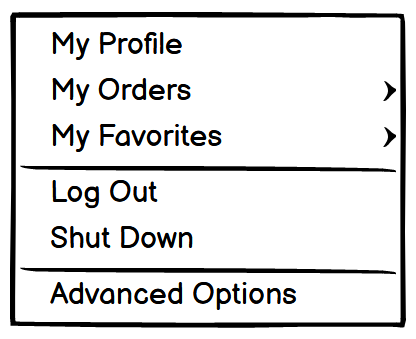
\includegraphics{h7-03}
\end{center}

\noindent\textbf{Example 2: The dialog indicates that ``cor launcher'' will be needed to ``associate files with Coral'' and that the user will need write permissions for the installation folder.}\\
\begin{center}
\noindent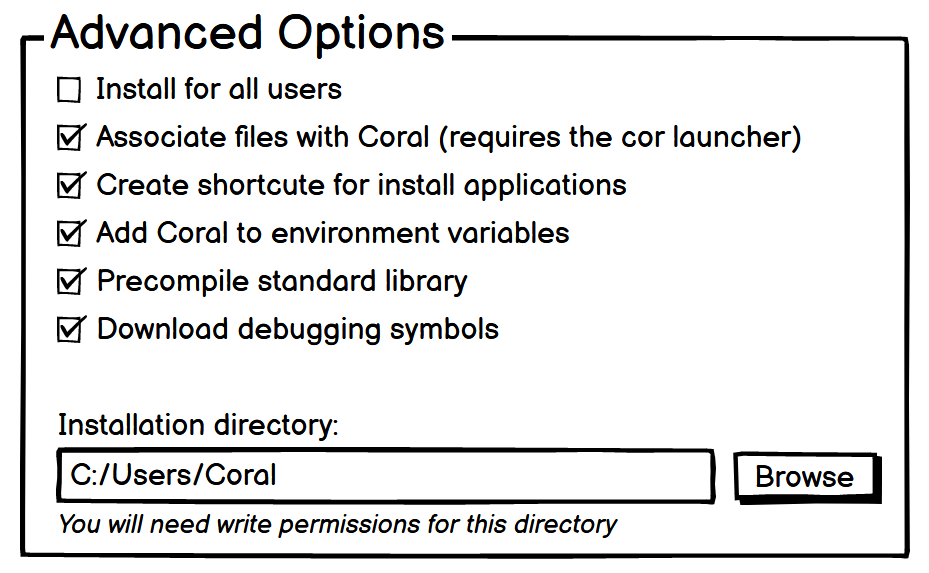
\includegraphics{h7-04}
\end{center}

\subsection{Heuristic \#3 (of 8): Let people gather as much information as they want, and no more than they want}

\begin{itemize}
\item Abi and Pat gather and read relevant information comprehensively before acting.
\item Tim likes to delve into the first option and pursue it, backtracking if need be.
\end{itemize}

\noindent To support their \textbf{information processing styles}, allow Abi and Pat to easily obtain as much information they want, but don't require them to spend excessive time or effort gathering that information. Allow Tim to get to directly useful information immediately so that they can act upon it without wading through a lot of information they don’t want.

\spacer
\noindent\textbf{Example 1: Users can choose to view code documentation while still viewing their code.}
\begin{center}
\noindent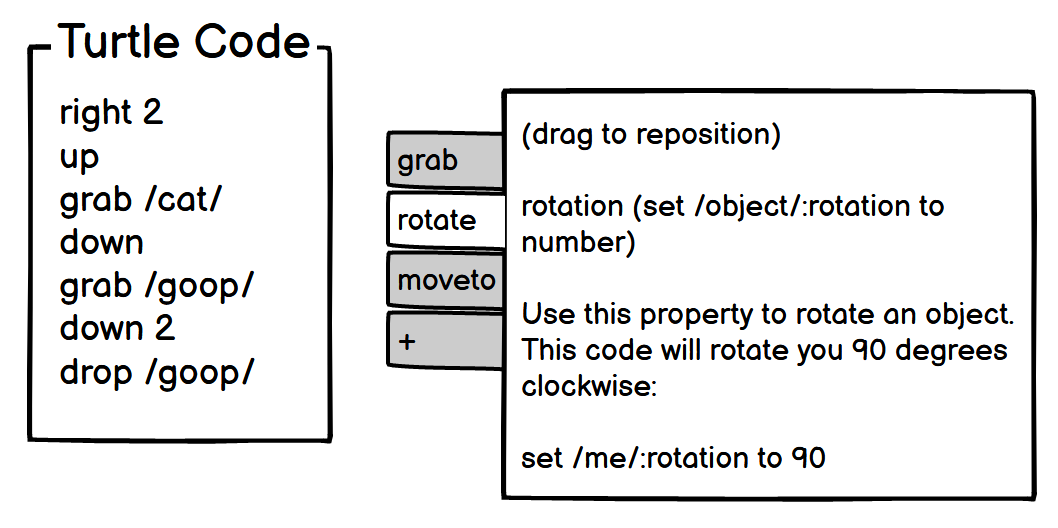
\includegraphics{h3-03}
\end{center}

\noindent\textbf{Example 2: Users can quickly see the contents of the webpage and jump to the section they're interested in.}
\begin{center}
\noindent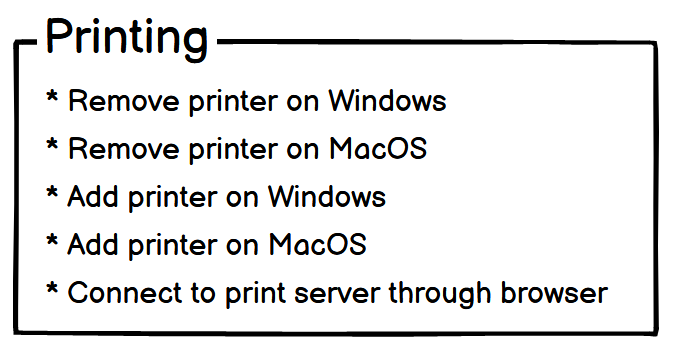
\includegraphics{h3-04}
\end{center}

\subsection{Heuristic \#4 (of 8): Keep familiar features available}

\begin{itemize}
\item Abi has lower computer self-efficacy and is more risk-averse than Tim, so if a problem arises when they are trying to use an unfamiliar feature, Abi blames themself and stops using the tech rather than potentially wasting their time trying to get the unfamiliar feature working.
\item Pat has medium self-efficacy with technology, so if a problem arises when they are trying to use an unfamiliar feature, Pat will try alternative ways of succeeding for a while. However, Pat is also risk-averse so prefers to perform tasks using familiar features, because they're more predictable about what Pat will get from them and how much time they'll take.
\item Tim has higher computer self-efficacy and is more risk-tolerant than Abi, so if a problem arises when they are trying to use an unfamiliar feature, they’ll blame the tech, and may spend a lot of extra time trying to work around a problem in numerous ways.
\end{itemize}

\noindent To support their \textbf{computer self-efficacies} and \textbf{attitudes toward risk}, and to encourage Abi, Pat, and Tim to keep using the tech without wasting their time, enable them to interact with it using the same features they’ve used in the past.

\spacer
\noindent\textbf{Example 1: Although the ``following'' page is gone, the new update looks similar to the previous version so that users are still familiar with the app.}
\begin{center}
\noindent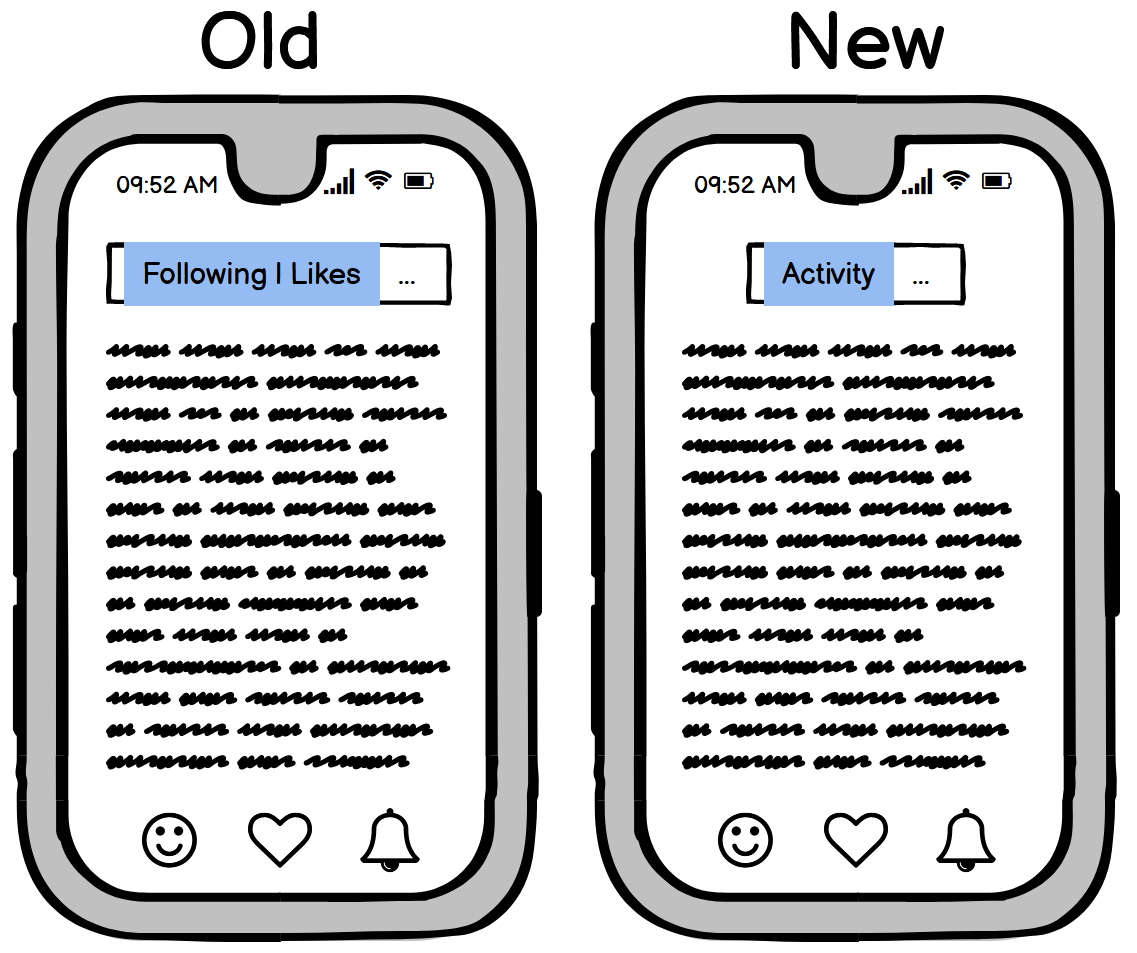
\includegraphics[width=0.7\textwidth]{h4-03}
\end{center}

\noindent\textbf{Example 2: The smartphone and tablet versions of this app offer the same features which makes switching between the two easy.}
\begin{center}
\noindent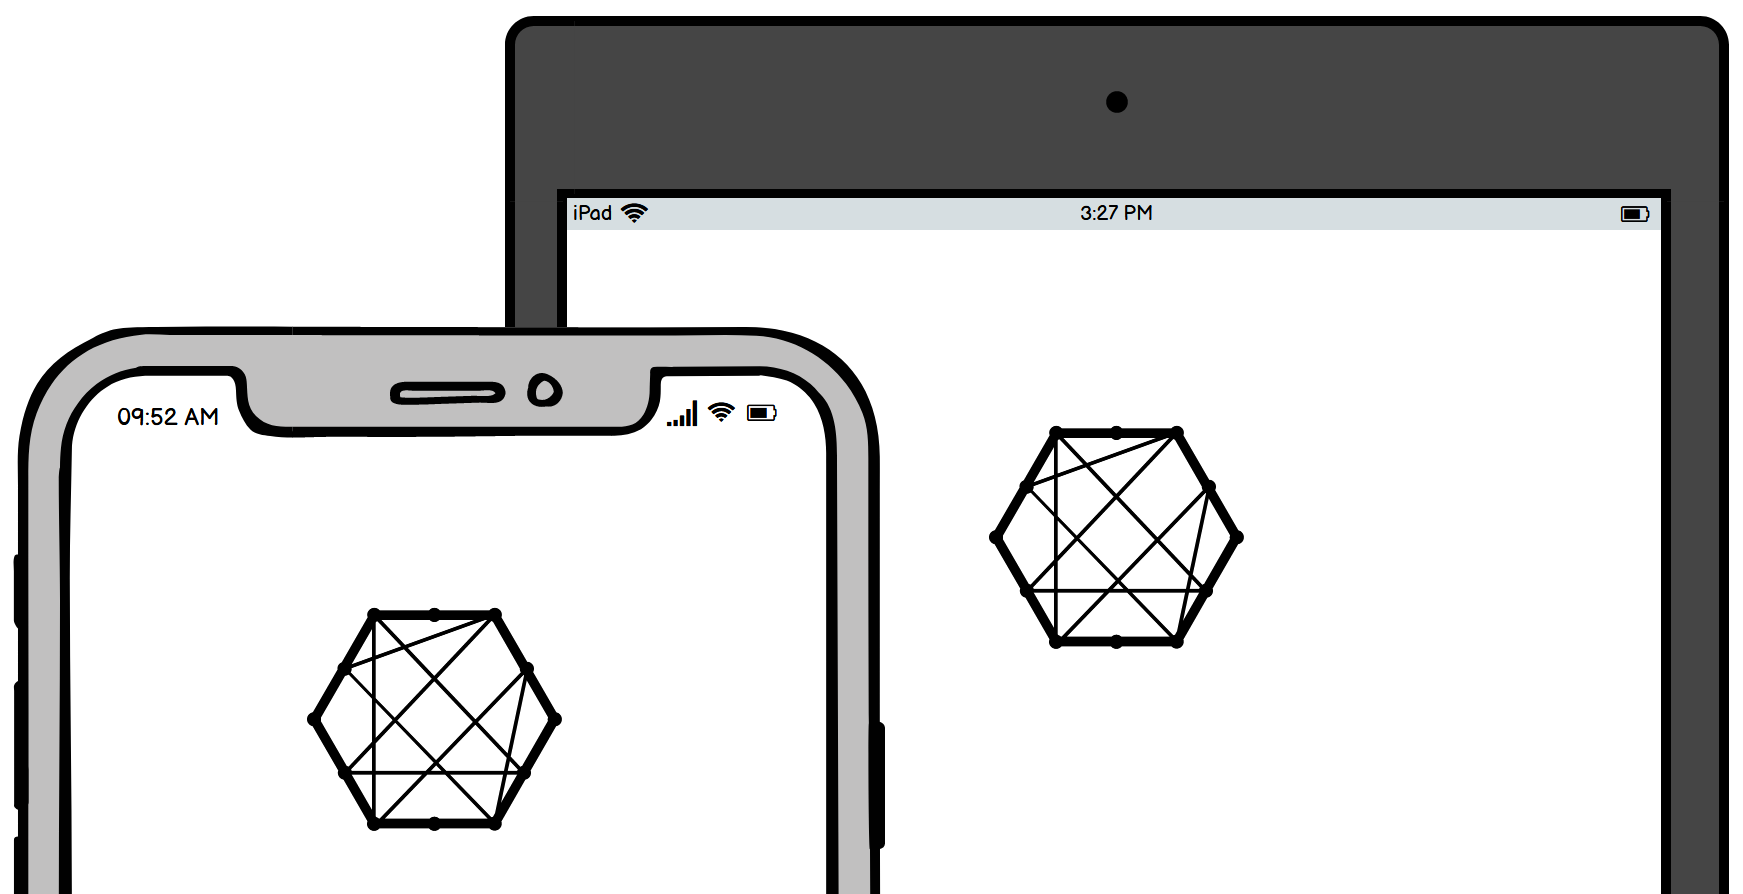
\includegraphics[width=0.7\textwidth]{h4-04}
\end{center}

\subsection{Heuristic \#5 (of 8): Make undo/redo and backtracking available}

\begin{itemize}
\item Abi and Pat are risk-averse, so they prefer not to take actions in technology that might not be easy to reverse.
\item Tim is risk-tolerant, so is willing to take actions in technology that might be incorrect and need to be reversed.
\end{itemize}

To support their \textbf{attitudes toward risk}, provide undo/redo and backtracking to allow Abi and Pat to feel comfortable proceeding with actions whose consequences may not be clear, so that that they know they can easily reverse these actions, and so that Tim can recover from mistakes.

\spacer
\noindent\textbf{Example 1: Browser back/forward buttons allow users to backtrack through their browsing history.}\\
\begin{center}
\noindent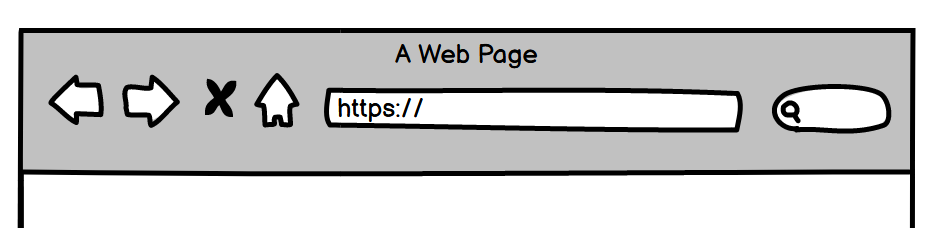
\includegraphics{h5-03}
\end{center}

\noindent\textbf{Example 2: An undo button allow users to make and recover from mistakes. Also, version control control systems allow users to revert to any previously-committed code state.}\\
\begin{center}
\noindent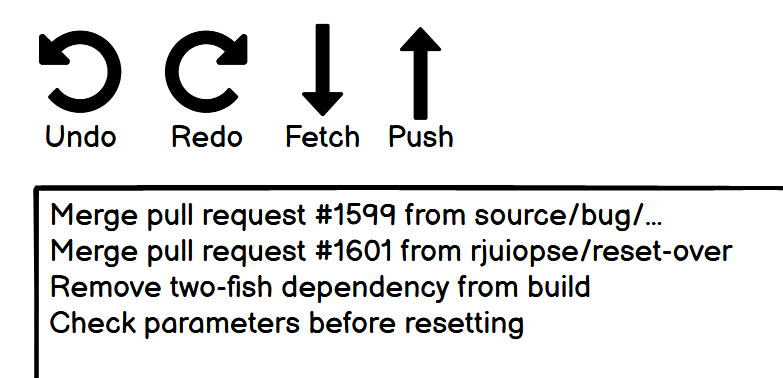
\includegraphics{h5-04}
\end{center}

\subsection{Heuristic \#6 (of 8): Provide an explicit path through the task}

\begin{itemize}
\item Abi is a process-oriented learner, so prefers to proceed through tasks step-by-step.
\item Tim and Pat learn by tinkering, and therefore prefer not to be constrained by rigid, pre-determined processes.
\end{itemize}

\noindent To support their \textbf{learning styles}, explicitly provide Abi a clear process to go through task, and provide Tim and Pat a way to bypass step-by-step processes and tutorials if those are not required for learning the technology.

\spacer
\noindent\textbf{Example 1: Users can choose their entry point, and each path is explained.}\\
\begin{center}
\noindent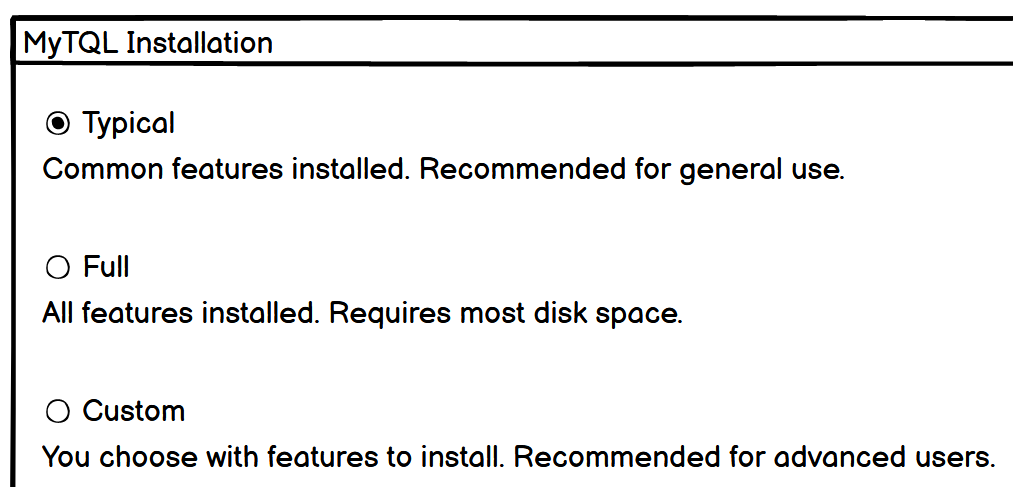
\includegraphics{h8-03}
\end{center}

\noindent\textbf{Example 2: Users get to choose either the path of learning more about the new feature or going back to what they were doing.}\\
\begin{center}
\noindent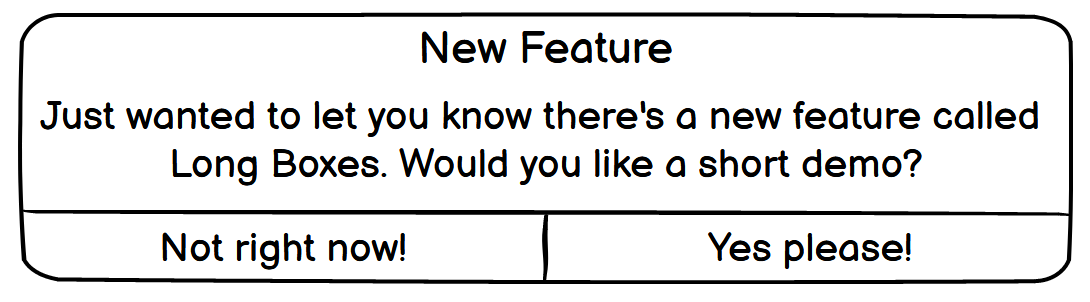
\includegraphics{h8-04}
\end{center}

\subsection{Heuristic \#7 (of 8): Provide ways to try out different approaches}

\begin{itemize}
\item Abi has lower computer self-efficacy than Tim, so if a problem arises when they are trying to use technology, Abi blames themself and stops using the tech.
\item Pat has medium self-efficacy with technology, so if a problem arises when they are trying to use technology,  Pat will try alternative ways of succeeding for a while.
\item Tim has higher computer self-efficacy than Abi, so if a problem arises when they are trying to use technology, they’ll blame the tech, and then will try numerous workarounds to get around the problem.
\end{itemize}

\noindent To support their \textbf{computer self-efficacies}, point Abi toward a different approach when they feel unable to proceed with the current one. This will also point Tim and Pat to multiple ways they can try to solve the problem.

\spacer
\noindent\textbf{Example 1: If users don't find what they need on the ``Choose a Question'' drop-down menu, they can try the chat.}\\
\begin{center}
\noindent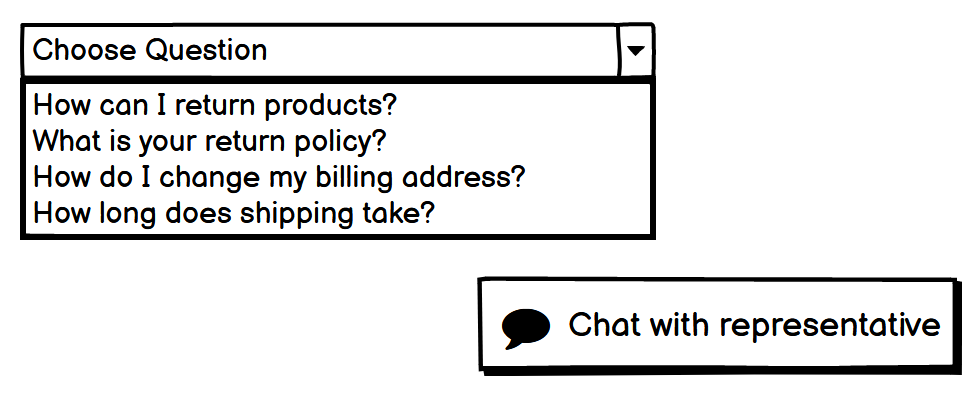
\includegraphics{h6-03}
\end{center}

\noindent\textbf{Example 2: If users encounter a problem using the SecureChat UI, they can attempt the same operations using the command line interface.}\\
\begin{center}
\noindent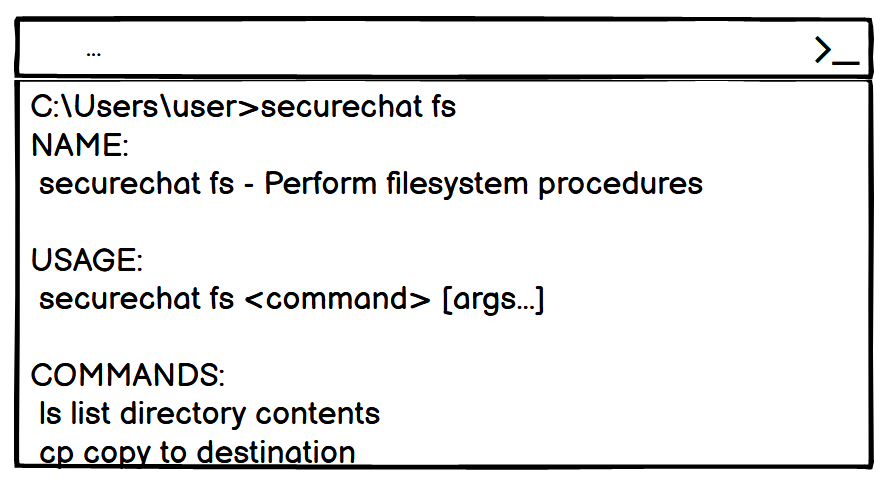
\includegraphics{h6-04}
\end{center}

\subsection{Heuristic \#8 (of 8): Encourage tinkerers to tinker mindfully}

\begin{itemize}
\item Tim learns by tinkering, but sometimes tinkers addictively and gets distracted from their task.
\item Pat learns by trying out new features but does so mindfully, reflecting on each step.
\end{itemize}

\noindent To support their \textbf{learning styles}, encourage Tim not to over-tinker (e.g., by adding an extra click), so that they make fewer mistakes, have time to absorb important information, and stay on-task.

\spacer
\noindent\textbf{Example 1: This design encourages users to tinker mindfully by showing they will notify them before impactful actions are executed, like emailing 237 people.}\\
\begin{center}
\noindent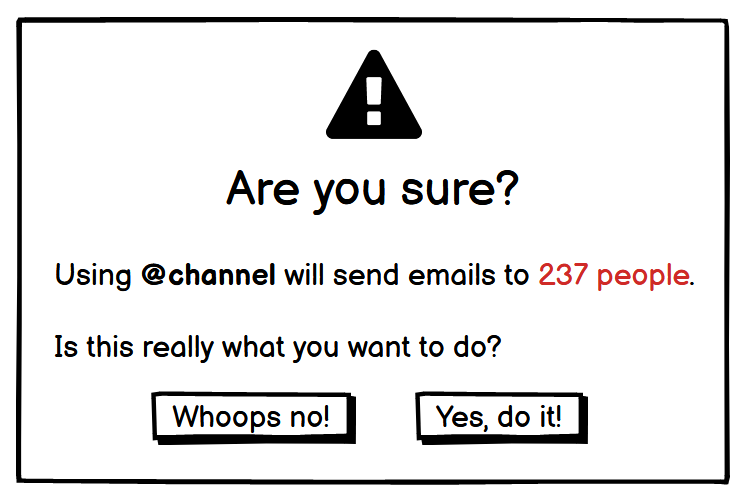
\includegraphics{h9-03}
\end{center}

\noindent\textbf{Example 2: This design encourages users to try out new ``slash'' commands by showing all the commands when a user types ``/'', and explaining what each does and how to use it.}\\
\begin{center}
\noindent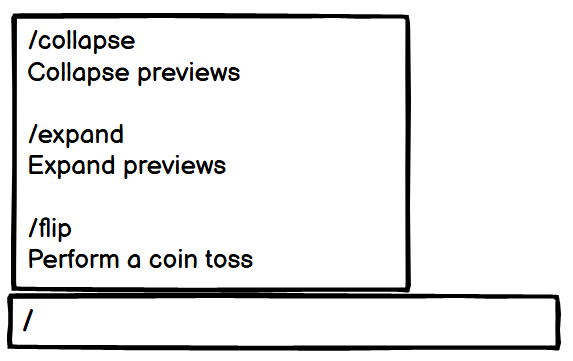
\includegraphics{h9-04}
\end{center}

\yesmargins
\section{Background}

\marginpar{\textbf{heuristic evaluation}: A usability inspection method where evaluators independently check that a design reflects a set of heuristics, then compare results \parencite{nielsen90}.\margindivider}

\marginpar{The cognitive style personas are simplified versions of the GenderMag personas. You can find the the GenderMag personas, and a full description of their research origins, at \href{http://gendermag.org/}{GenderMag.org}\margindivider}

\marginpar{\textbf{GenderMag Method:} A method for finding and fixing gender-inclusivity bugs in software that uses a specialized cognitive walkthrough and the customizable Abi, Pat, and Tim personas \parencite{burnett16}\margindivider}

\marginpar{\textbf{cognitive walkthrough\index{cognitive walkthrough}}: A usability inspection method that involves stepping through a user interface as a user, stopping to ask specific questions about the user's experience \parencite{nielsen94}.}

The Cognitive Style Heuristics are meant to be used in a \textbf{heuristic evaluation}\index{heuristic evaluation}, a process where software designers or evaluators go through heuristics one-by-one like a checklist, deciding whether the design does or does not reflect the heuristic. The evaluation is done independently by two or more people, who then compare findings.

The Cognitive Style Heuristics are derived from the GenderMag Heuristics \parencite{gendermagheuristics} and the \textbf{GenderMag Method} \parencite{burnett16}. The GenderMag Method a process for finding and fixing gender-inclusivity bugs in software. Instead of heuristic evaluation, it uses a \textbf{cognitive walkthrough}. It uses the same personas: Abi, Pat, and Tim. However, in addition to their cognitive styles, each GenderMag persona has additional sections, such as one with customizable background information.

What do cognitive styles have to do with gender? Software tends to be biased against the cognitive styles often favored by women. Designing with cognitive styles in mind can make software less gender-biased \parencite{vorvoreanu19}.

In addition, ``designing software so that it works for diverse populations matters to software companies’ profitability, to equity in the workplace and at home, and to anyone in a situation that changes the way they think, such as when under deadline pressure.''\parencite{mendez19}

\section{Conclusion}

The Cognitive Style Heuristics are a set a eight software usability heuristics for evaluating and improving the usability of UIs across users with different cognitive styles.

\nomargins
\section{Additional Resources}

\begin{description}
\item \fullcite{burnett16}
\item \fullcite{hill2017gender}
\item \fullcite{gendermag}
\item \fullcite{gendermagheuristics}
\item \fullcite{martin12}
\item \fullcite{mendez19}
\item \fullcite{nielsen90}
\item \fullcite{nielsen94}
\item \fullcite{norman13}
\item \fullcite{pruitt10}
\item \fullcite{vorvoreanu19}
\end{description}